% Ch5.tex

\chapter[Multiple-instance multiple-label learning for the classification of frog calls with acoustic event detection]{Multiple-instance multiple-label learning for the classification of frog calls with acoustic event detection}
\label{cha:cha6MIML}


\section{Introduction}
\label{sec:intro}

This chapter presents a method for the classification of simultaneously vocalising frog species in low SNR recordings. In chapter 4 and 5, frog call classification is solved using a SISL framework, which cannot reflect the nature of the low SNR recordings. Most low SNR recordings often 
contain multiple overlapping animal vocal activities including frogs, birds, crickets and so on. To solve this problem, the multiple-instance multiple-label framework for supervised classification is formulated.

A representative sample of 342 10-seconds recordings was exported from the database and split into testing and training sets. The performance is evaluated based on the MIML learning measures. Experimental results demonstrate the MIML classification framework can be adopt to classify multiple simultaneously vocalising frog species in low SNR recordings.


\section{Conference paper - }

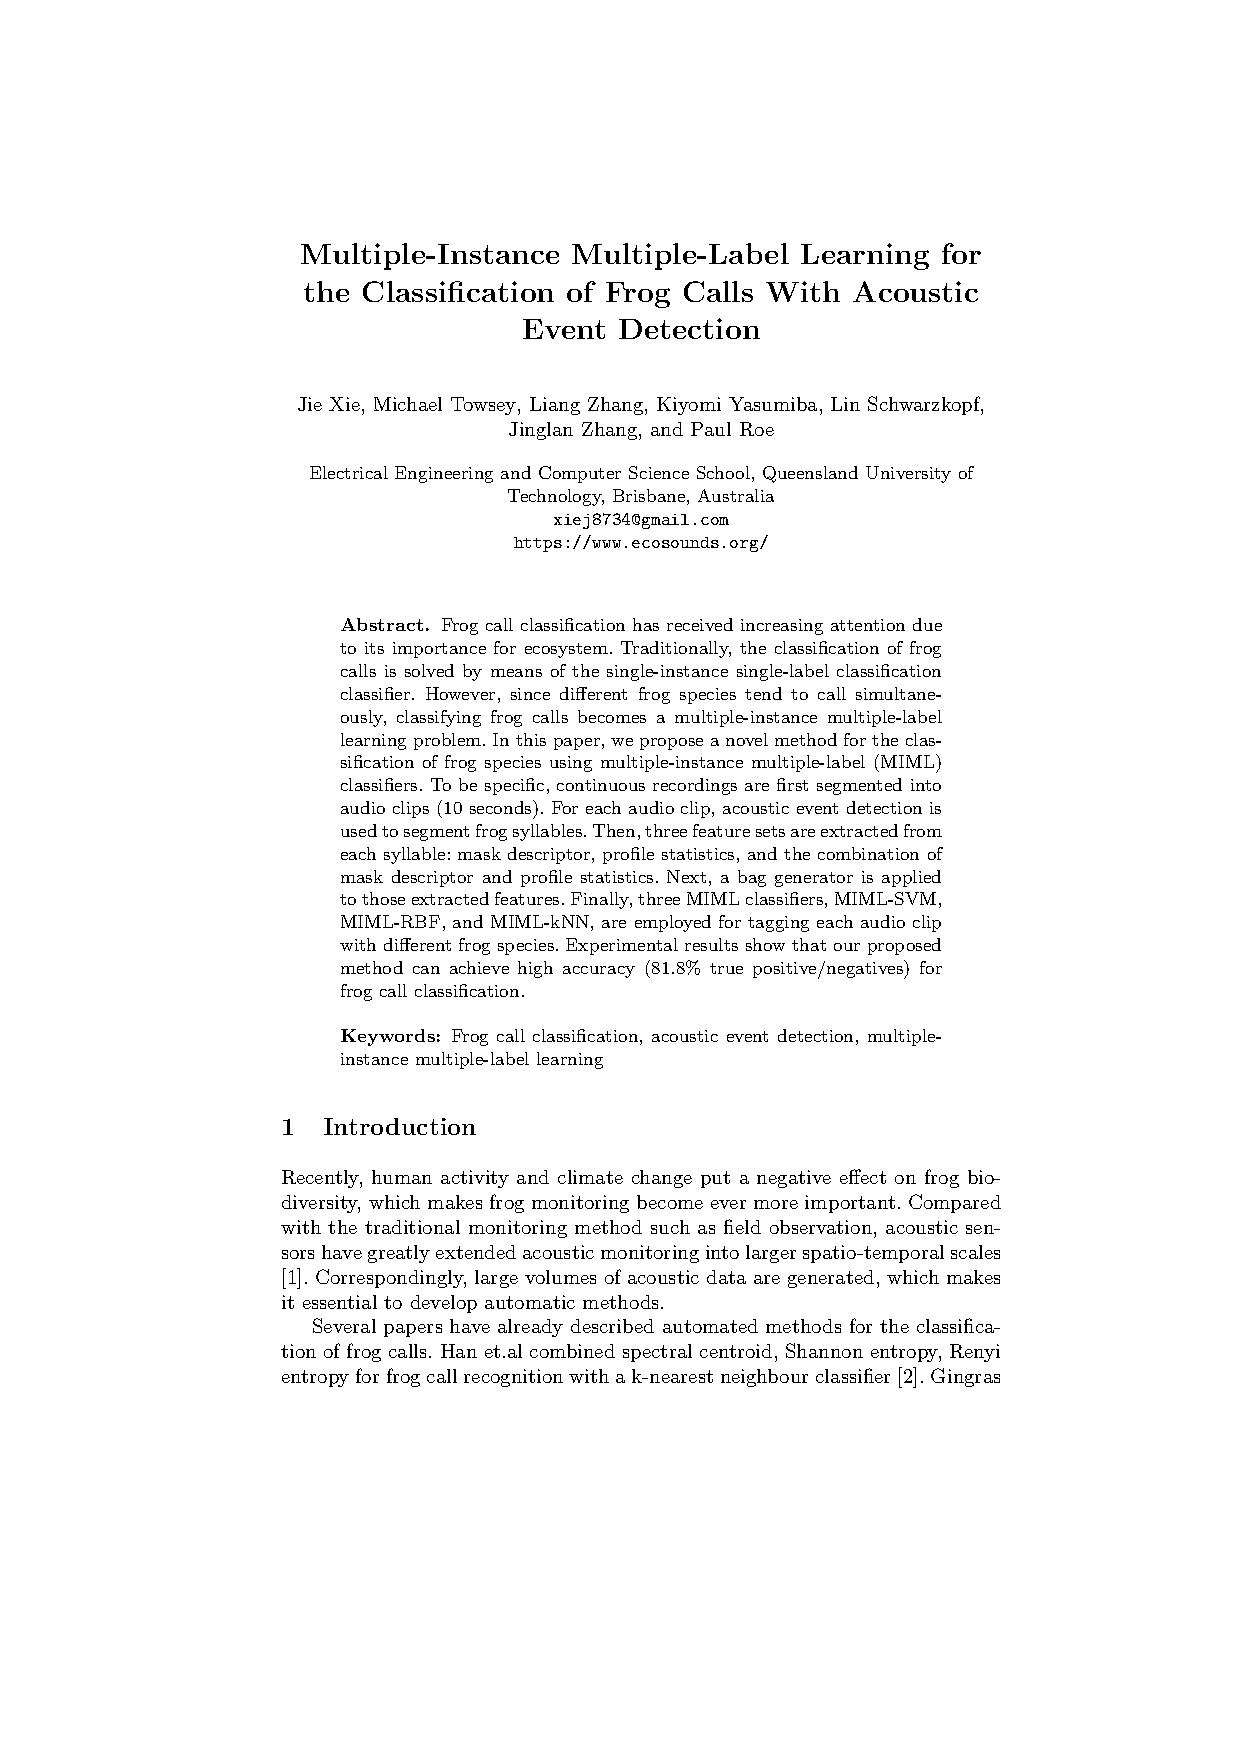
\includepdf[pages=-, pagecommand={},width=1.5\textwidth]{Ch6_paper.pdf}

